网约车个体补贴分配是在预算约束下，最大化业务目标。其优化问题为多选择背包问题（multiple-choice knapsack problem, MCKP）\citep{boyd2004convex}
。\subsection{原问题$P_1$}
原问题本质上是一个带约束的0-1整数规划问题：
\textbf{定义}：

\begin{equation} \label{eq:mckp}
\begin{aligned}
\max_{\bm{z}} \quad & \sum_{i} \sum_{j} v_{ij} z_{ij} \\
\text{s.t.} \quad & \sum_{i}\sum_{j} c_{ij} z_{ij} \le B  \\
& \sum_{j} z_{ij} = 1, \quad \forall i \\
& z_{ij} \in \{0, 1\}, \quad\forall i,\forall j
\end{aligned}
\end{equation}
\begin{itemize}
    \item $i$：表示每一条定价样本，即冒泡
    \item $j \in J$：表示待选的折扣
    \item $v_{ij}$：表示冒泡$i$在折扣 $j$下的收益
    \item $c_{ij}$：表示冒泡$i$在折扣 $j$下的补贴金额
    \item $z_{ij}$：决定对于冒泡$i$是否选择折扣$j$的决策变量
    \item $B$：表示总补贴额
\end{itemize}

\par
该整数规划问题为NP-Hard（无已知多项式时间复杂度的精确解），并且在整数规划问题中，决策变量是离散的点导致问题不可微分，无法使用最优性条件（例如KKT条件）直接求解\citep{hartmanis1982computers}。\par
优化问题\eqref{eq:mckp}的近似求解方法主要有两种：贪心算法 \citep{sinha1979multiple}和对偶松弛 \citep{fisher1981lagrangian}，两者得到的整数解都是近似最优。设理论最优值为$OPT$，所有冒泡的$v_{ij}$中最大值为$\max_{ij}v_{ij}$，这两种近似算法\citep{sinha1979multiple, fisher1981lagrangian}解的效果和理论最优的近似比$\nu$为：
$\nu = 1-\frac{\max_{ij}v_{ij}}{OPT}$。



\subsection{贪心算法求解\citep{sinha1979multiple}}

\subsubsection{线性松弛}
直接求解原整数规划问题（Integer Programming）属于NP-Hard问题，计算成本极高。Sinha等人通过引入线性松弛（Linear Relaxation）结合贪心算法近似求解，其中引入线性松弛主要基于以下目的：
\begin{enumerate}
    \item \textbf{决策空间剪枝：} 通过线性松弛的凸性分析，可以识别出次优的决策变量。这些决策变量在最优解中必然为0，因此可在预处理阶段被剔除，缩小问题规模 \citep{sinha1979multiple}。

    \item \textbf{线性松弛解仅有一个冒泡的决策变量为分数：} Sinha和Zoltners证明，该问题的线性松弛解具有特殊性质（线性松弛问题的解中最多有一个冒泡的决策变量为分数）。这允许采用贪心算法快速求得松弛解，而无需使用单纯形法对复杂的原整数规划问题求解 \citep{sinha1979multiple}。
    
\end{enumerate}


松弛后的问题如下：
\begin{equation} \label{eq:smckp}
\begin{aligned}
\max_{\bm{z}} \quad &  \sum_{i} \sum_{j} v_{ij} z_{ij} \\
\text{s.t.} \quad & \sum_{i}\sum_{j} c_{ij} z_{ij} \le B  \\
& \sum_{j} z_{ij} = 1, \quad \forall i \\
& z_{ij} \in [0, 1]，\quad \forall i,\forall j
\end{aligned}
\end{equation}\par





\subsubsection{决策空间剪枝}

在进行求解前，对于个体$i$，有明显不在最优解内的的决策变量$z_{is}$，可以直接取0。
类别1同时适用于原问题P1和线性松弛问题P2，类别2依赖于线性组合只适用于P2 \citep{sinha1979multiple}。





\paragraph{类别1: k-dominated（k类次优决策变量）}
对于同一冒泡 $i$ 的两个不同折扣 $j, k$，若满足：
$$ c_{ij} \le c_{ik} \quad \text{且} \quad v_{ij} \ge v_{ik} $$
则在最优解中$z_{ik}=0$。

\textcolor{red}{若成本大却收益小，则该解一定不是最优解，可以提前排除}

\paragraph{类别2: p-dominated（p类次优决策变量）}
经过类别1剪枝后，对于$c_{ir} < c_{is} < c_{it}$（$r, s, t \in R_i$），有$v_{ir} < v_{is} < v_{it}$。进一步考察边际收益率（斜率），若满足：
\begin{equation}
\frac{v_{is} - v_{ir}}{c_{is} - c_{ir}} < \frac{v_{it} - v_{is}}{c_{it} - c_{is}}
\end{equation}
则$z_{is}$不是最优解，即$z_{is}=0$，可被剪枝。
\\

\textcolor{red}{随着补贴增加，补贴的ROI应该边际递减（即ROI的一阶导永小于等于零）。若一阶导函数存在正值，则该解一定不是最优解，可以提前排除}

\textbf{证明\citep{sinha1979multiple}:}
分子分母均为正数时，若：
\begin{equation}
\frac{a}{b}<\frac{c}{d}
\end{equation}
则
\begin{equation}
\frac{a}{b}<\frac{a+c}{b+d}<\frac{c}{d}
\end{equation}
公式3代入
得：
\begin{equation}
\frac{v_{is} - v_{ir}}{c_{is} - c_{ir}} <\frac{v_{it} - v_{ir}}{c_{it} - c_{ir}}< \frac{v_{it} - v_{is}}{c_{it} - c_{is}}
\end{equation}
这意味着点 $(c_{is}, v_{is})$ 位于连接点 $(c_{ir}, v_{ir})$ 和 $(c_{it}, v_{it})$ 的线段下方。即直接通过 $r$ 和 $t$ 的线性组合，可以在消耗同样成本的情况下获得比 $s$ 更高的收益。因此$z_{is}$一定为0。
\par
考虑冒泡$i$下一组共$J$个决策，对应的$v_{ij}$和$c_{ij}$，不满足“命题1”和“命题2”的折扣一定不在最优解中，对应的决策变量一定为0，用$\bm{J'}$表示剪枝后折扣集合。即可以写成：
\begin{equation}
\begin{aligned}
0 \leq v_{i1} \leq v_{i2} \leq \dots \leq v_{ij'}\quad \forall i\\
0 \leq c_{i1} \leq c_{i2} \leq \dots \leq c_{ij'} \quad \forall i\\
 \frac{v_{i2} - v_{i1}}{c_{i2} - c_{i1}} \geq \frac{v_{i3} - v_{i2}}{c_{i3} - c_{i2}} \geq \dots \geq \frac{v_{ij'} - v_{i(j'-1)}}{c_{ij'} - c_{i(j'-1)}} \quad \forall i
\end{aligned}
\end{equation}


\begin{figure}[!h]
    \centering
    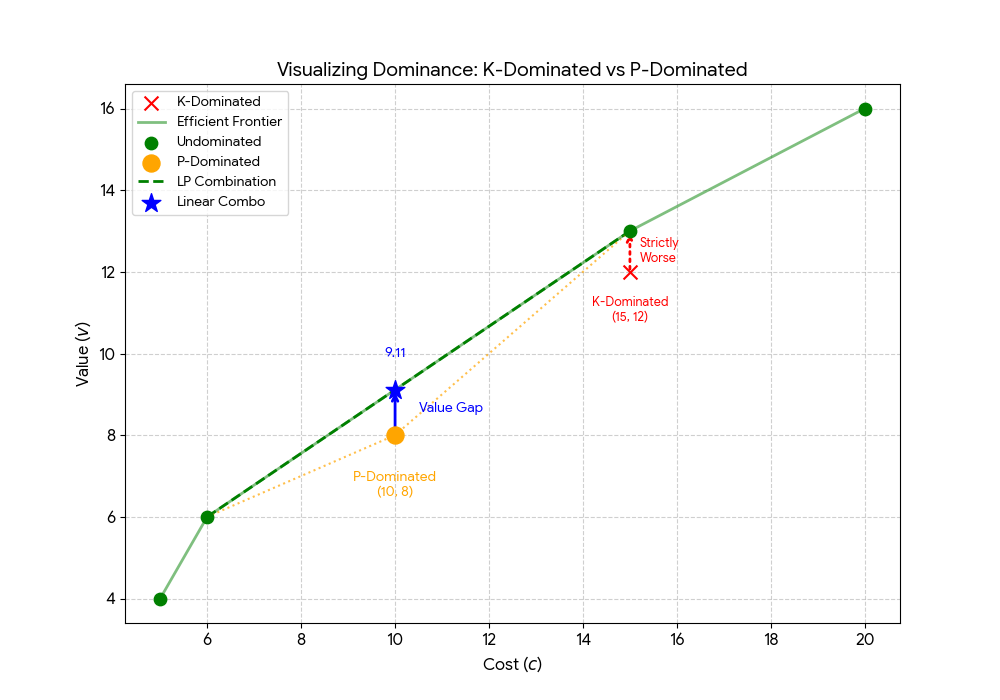
\includegraphics[width=5in]{figures/dominance_final_clean.png}
    \caption{类别1:k-dominated和类别2:p-dominated}
    \label{fig:my_label}
\end{figure}\par
将每个冒泡 $i$ 的决策过程视作从最低成本开始的增加补贴过程。\\
对于$j=1$，$\sum_i{c_{i1}}<B$否则问题P1、P2的可行域都是空集。
对于$j>1$当冒泡 $i$ 当前处于第 $j-1$ 档折扣，若将其增加补贴到第 $j$ 档折扣：
\begin{itemize}
    \item 边际成本增量：$\Delta c_{ij} = c_{ij} - c_{i(j-1)}\quad \forall i$
    \item 边际收益增量：$\Delta v_{ij} = v_{ij} - v_{i(j-1)}\quad \forall i$
\end{itemize}

定义该动作的\textbf{投资回报率(Return On Investment，ROI)}为：
\begin{equation}
\rho_{ij} = \frac{\Delta v_{ij}}{\Delta c_{ij}}\quad\forall i\quad \forall j
\end{equation}


%\textcolor{red}{命题2的intuition是什么？这个有什么作用（为什么放在这里）？是公认（通用）的吗？证明是你证的，还是已有文献给出的。给出文献}


\subsubsection{全局排序与贪心选择}
将所有冒泡的所有潜在加补动作(假设最初所有冒泡都给最小的补贴额$c_{i1},\forall i$,此时一定有$\sum_ic_{i1}<B$，记$c_{i(j'-1)}$ 到$c_{ij'}$为一次加补动作，$\forall j'>1$)放入一个全局集合，记为 $S_{all}$：
$$ S_{all} = \{ (i, j') \mid \forall i, \forall j'>1 \} $$\par
按照 $\rho_{ij}$ 从大到小对集合 $S_{all}$ 进行排序，得到有序序列：
$$ \text{Seq} = \{ \text{step}_1, \text{step}_2, \dots, \text{step}_N \} $$\par
其中 $\rho(\text{step}_k) \ge \rho(\text{step}_{k+1})$。

线性松弛问题 $P_2$ 的求解等价于：\textbf{按顺序执行这些升级动作，直到预算 $B$ 耗尽。}
设 $C_k$ 为执行前 $k$ 个动作的累计成本。由于预算有限，必然存在一个点$m$，使得：
\begin{equation}
C_{m-1} \le B < C_m
\end{equation}

\subsubsection{解的结构}
根据上述贪心过程，最优解 $\bm{z}^*$ 的取值被点 $m$ 划分为三类：

\begin{enumerate}
    \item \textbf{为1的部分} ($k < m$)：
    排序在点$m$之前的升级动作被执行。对于这些动作所属的冒泡，其决策变量最终停留在某个确定的高档位，即 $z_{ij} = 1$（整数）。

    \item \textbf{为0的部分} ($k > m$)：
    排序在点$m$之后的动作因预算不足被放弃。对应的高档位决策变量 $z_{ij} = 0$（整数）。

    \item \textbf{为分数的部分} ($k = m$)：
    这是唯一发生“预算耗尽”时刻的动作。为了花完剩余预算 $(B - C_{m-1})$，只能部分选取 $m$ 。
    该动作对应的冒泡 $i^*$ 是全局唯一取值为分数的样本。$m$对应的$v$也就是P1\eqref{eq:mckp}和P2\eqref{eq:smckp}的松弛间隙。
\end{enumerate}

\subsubsection{结论与近似误差}
综上所述，线性松弛解 $\bm{z}_c^*$ 在结构上仅包含一个分数项，其余均为整数。
令 $F_{\bm{z_c^*}}$ 为线性松弛最大收益，$F_{z^*}$ 为整数规划最大收益。由于仅有第 $m$ 个动作为分数，两者之差不会超过该动作带来的最大可能收益 $v_{max}$，因此两者之差的上界如下：
\begin{equation}
F_{\bm{z_c^*}} - F_{\bm{z^*}} < v_{\max}
\end{equation}\par
考虑到网约车场景下总收益 $F_{\bm{z^*}}$ 远大于单个收益 $v_{\max}$，因此该近似带来的相对误差趋近于0，如下所示:
\begin{align}
    \lim_{N\to \infty} F_{\bm{z^{*}}} - F_{\bm{z^*_c}} = 0
\end{align}

因此线性松弛解$\bm{z_c^*}$的整数部分可以视作原整数问题的最优解。
贪心算法将线性松弛问题的求解复杂度降低到了$\mathcal{O}\left(N\log \|J\| + N \log N +N \right) = \mathcal O (N\log N)$。
然而，当$N$极大时，求解速度仍较慢。因此，为进一步提升求解速度，可通过拉格朗日松弛，将该预算约束问题转化为无约束问题进行求解。



\subsection{拉格朗日对偶问题P3}

拉格朗日对偶将 NP-Hard 问题分解为易解的子问题。

\subsubsection{拉格朗日函数}

线性松弛问题 \eqref{eq:smckp} 的约束分为两类：
\begin{enumerate}
    \item 不等式约束（预算约束）：$\sum_{i}\sum_{j} z_{ij} \cdot c_{ij} - B \leq 0$
    \item 等式约束（每个个体选且仅选一个处理）：$\sum_{j} z_{ij} - 1 = 0, \forall i$
\end{enumerate}


附录证明了对于等式约束可以不松弛，解的效果是等价的。
因此在构造拉格朗日函数（Lagrangian Function）$L(\bm z,\lambda)$时只对不等式约束进行松弛，得到拉格朗日函数$L(\bm{z},\lambda)$：
\begin{align}
L(\bm{z}, \lambda) &= \sum_{i}\sum_{j} z_{ij} \cdot v_{ij} - \lambda \cdot \left( \sum_{i}\sum_{j} z_{ij} \cdot c_{ij}-B\right)\\
&= \sum_{i}\sum_{j} z_{ij} \cdot v_{ij} + \lambda B - \lambda \sum_{i}\sum_{j} z_{ij} \cdot c_{ij}  \\
&= \sum_{i}\sum_{j} z_{ij} \cdot (v_{ij} - \lambda \cdot c_{ij} ) + \lambda \cdot B 
\end{align}
\subsubsection{对偶函数}
对偶函数 $D(\lambda)$ 是关于$\lambda$的函数，
定义为：给定 $\lambda$ 时，$L(\bm{z}, \lambda)$ 关于 $\bm{z}$ 的最大值：

\begin{align}\label{eq:dualfunction}
D(\lambda) &= \max_{\bm{z}} L(z, \lambda) \\
&= \max_{\bm{z}} \left( \sum_{i}\sum_{j} z_{ij} \cdot (v_{ij} - \lambda \cdot c_{ij} ) + \lambda \cdot B  \right)\\
&= \lambda \cdot B + \underbrace{\max_{\bm{z_1}}  \sum_{j} z_{1j} \cdot (v_{1j} - \lambda \cdot c_{1j} ) + \cdots + \max_{\bm{z_N}}  \sum_{j} z_{Nj} \cdot (v_{Nj} - \lambda \cdot c_{Nj} )}_{\sum_{i}\max_{\bm{z_{i}}} \left(\sum_{j} z_{ij} \cdot (v_{ij} - \lambda \cdot c_{ij} ) \right)}\\
&=  \lambda \cdot B +\sum_{i}\max_{\bm{z_{i}}} \left(\sum_{j} z_{ij} \cdot (v_{ij} - \lambda \cdot c_{ij} ) \right) 
\end{align}

要使$L(\bm z,\lambda)$取最大值，需对每个个体 $i$ 选择能最大化 $(v_{ij} - \lambda c_{ij})$ 的处理 $j$：

令：
\begin{equation}
j^{*}(i, \lambda) = \arg\max_{j} (v_{ij} - \lambda \cdot c_{ij})
\end{equation}

\textbf{定义对偶函数解：}
对于给定的$\lambda$ 确定的决策变量  $\bm{z^d} = \{z_{ij}^d\}$ 为：
$$z_{ij}^d = 
\begin{cases} 
1 & \text{if } j = j^*(i,\lambda)\\ 
0 & \text{otherwise} 
\end{cases}$$
把$\bm {z^d}$代入$\eqref{eq:dualfuncation}$，可得：

\begin{equation}\label{eq:Dlambda}
\begin{aligned}
D(\lambda)&=\lambda \cdot B + \sum_i(v_{ij^*(i,\lambda)}-\lambda \cdot c_{ij^*(i,\lambda)})\\
&= \lambda \cdot \left( B-\sum_{i} c_{ij^*(i,\lambda)} \right) + \sum_{i} v_{ij^*(i,\lambda)}
\end{aligned}
\end{equation}

\subsubsection{对偶问题}
基于对偶函数$D(\lambda)$ \eqref{eq:Dlambda}，其对应的对偶问题如下所示：
\begin{equation}\label{eq:dual_problem}
\min_{\lambda \ge 0} D(\lambda)
=\min_{\lambda \ge0}\left(\lambda \cdot \left(B-\sum_ic_{ij^*(i,\lambda)}\right)+\sum_iv_{ij^*(i,\lambda)}\right)
\end{equation}

该问题的最优解可通过求导得到。然而，由于\eqref{eq:dual_problem}中$j^*(i,\lambda)$为分段线性函数，所以对偶函数$D(\lambda)$存在不可导的点。

常用的替代方案为用次梯度进行求导计算\citep{boyd2004convex}。$D(\lambda)$的次梯度如下所示：
\begin{align}
D'(\lambda) &= \frac{\partial D(\lambda)}{\partial \lambda} \\
&=  B-\sum_{i} c_{ij^*(i,\lambda)}
\end{align}
$\lambda^*$可在$D'(\lambda)=0$时求得。

为求解 $D'(\lambda) \approx 0$，常见两种数值方法，分别为（1）梯度下降法以及（2）二分法。下文对两种方法进行介绍。

\paragraph{方法一：梯度下降法 (Gradient Descent)}
此方法利用梯度方向逐步更新 $\lambda$，直到总成本逼近预算 $B$（因目标是最小化，改用梯度下降）。
\begin{algorithm}[H]
\caption{梯度下降求解 $\lambda^*$}
\begin{algorithmic}[1]
\State 初始化：$\lambda=0$，学习率$\alpha$，误差阈值$\epsilon$，目标$B$
\State 计算 $j^*_i = \underset{j}{\operatorname{argmax}} (v_{ij} - \lambda c_{ij}), \forall i$，并求 $C_{\text{total}} = \sum_i c_{ij^*_i}$
\While{$|B - C_{\text{total}}| \ge \epsilon$}
    \State $\lambda = \lambda - \alpha \cdot (C_{\text{total}} - B)$ 
    \State 更新 $j^*_i$ 和 $C_{\text{total}}$（同步骤2）
\EndWhile
\State \Return $\lambda^* = \lambda$
\end{algorithmic}
\end{algorithm}

\paragraph{方法二：二分法 (Bisection Method)}
由于 $h'(\lambda)$ 关于 $\lambda$ 单调递减（$\lambda$ 越大，选的补贴方案成本越低，总成本越低），使用二分法快速逼近零点。

\begin{algorithm}[H]
\caption{二分法求解 $\lambda^*$}
\begin{algorithmic}[1]
\State 初始化：$\lambda_{\text{left}}=0$, $\lambda_{\text{right}}= \max\limits_{i,j}\frac{v_{ij}}{c_{ij}}$, $\epsilon$ (误差阈值)，目标预算$B$
\While{$\lambda_{\text{right}} - \lambda_{\text{left}} \ge \epsilon$}
    \State $\lambda_{\text{mid}} = (\lambda_{\text{right}} + \lambda_{\text{left}})/2$
    \State 计算 $j^*(i,\lambda) = \underset{j}{\operatorname{argmax}} \left( v_{ij} - \lambda_{\text{mid}} c_{ij} \right), \forall i$
    \State $C_{\text{total}} = \sum_i c_{ij^*(i,\lambda)}$
    \State $h'(\lambda_{\text{mid}}) =  B - C_{\text{total}} $
    \If{$h'(\lambda_{\text{mid}}) \ge 0$}
        \State $\lambda_{\text{right}} = \lambda_{\text{mid}}$ \Comment{预算剩余，需减小$\lambda$}
    \Else
        \State $\lambda_{\text{left}} = \lambda_{\text{mid}}$ \Comment{成本超支，需增大$\lambda$} 
    \EndIf
\EndWhile
\State \Return $\lambda^* = (\lambda_{\text{left}} + \lambda_{\text{right}})/2$
\end{algorithmic}
\end{algorithm}
\subsubsection{对偶问题最优解}
在通过上述方法解出来最优的$\lambda^*$后，对应的决策变量$\bm z^{d}(\lambda^*)$:
\begin{align}
z_{ij}^{d*} = 
\begin{cases}
1, & \text{if } j = \arg\max\limits_{j} \left( v_{ij} - \lambda^* \cdot c_{ij} \right) \\ 
0, & \text{otherwise} 
\end{cases}
\end{align}

Slater条件：对于一个凸问题，若不等式约束为仿射约束，只要可行域非空，那么该凸问题和它的对偶问题一定是强对偶,即
\begin{align}
F(\bm z^d(\lambda^*)) = F(\bm z_c^{*})
\end{align}

该线性松弛问题满足Slater条件，具有强对偶性：
\begin{align}
F(\bm z^d(\lambda^*)) = F(\bm z_c^{*}) 
\end{align}

由\eqref{eq10}可知整数规划问题和线性松弛问题的松弛间隙有界

\begin{align} 
F(\bm z^*)\leq F(\bm z_c^*)\leq F(\bm z^*) + \max_{i,j} v_{ij}
\end{align}
因此对偶求解的结果和整数规划问题的近似比为\par
$$1\leq \frac{F(\bm z^d(\lambda^*))}{F(\bm z^*)}\leq 1+\max_{ij}\frac{v_{ij}}{F(z^*)}$$